%---------------------------------------------------------------------------
% A0 Poster Using cfpposter style
%---------------------------------------------------------------------------

%---------------------------------------------------------------------------
% --- Preamble
%---------------------------------------------------------------------------
\documentclass[a0,portrait]{a0poster}
\usepackage{times}
\usepackage{cfpposter}
\usepackage[utf8]{inputenc} % Only if you need international characters
\usepackage{multicol}
%\usepackage{float}
\usepackage{amsfonts, amsmath, amsthm, amssymb} %
\usepackage{bm} % Math bold face
\usepackage{bbm}
\DeclareMathOperator{\Tr}{Tr} % Trace operator
%\usepackage{amssymb}
%\usepackage[pdf]{pstricks}


%%%%%%%%%%%%%%%%%%%%%%%%%%%%%%%%%%%%%%%%%%%%%%%%%%%%%%%%%%%%%%%%%%%%%%%%%%%%%
%%%%%%%%%%%%%%%%%%%%%%%%%%%%%% User specified LaTeX commands.
\usepackage{braket}

\usepackage{babel}

\begin{document}

%---------------------------------------------------------------------------
% --- Front Matter
%---------------------------------------------------------------------------

% The title of your poster:
\title{Quantum Monte Carlo Simulations of the Hubbard Model}

% The author(s)
\author{Francisco M. O. Brito, Jo\~ao M. V. P. Lopes, and Eduardo V. Castro}
\vspace{-2cm}
% The affiliation(s). You can use the macro \cfpaddress or fill in any other
% appropriate address.
\affiliation{\cfpaddress}

% Your email:
\email{francisco.brito@fc.up.pt}

% Whatever you want to put in the footer box
\thanks{\hfill \Wemail \hfill $\bullet$ \hfill JEFFA III 2018 \hfill $\bullet$ \hfill  \hfill}

\makeheader


%---------------------------------------------------------------------------
% --- The Poster Contents
%---------------------------------------------------------------------------

% You can choose how many columns you want by setting the second argument 
% below to that number. The multicol package distributes the text automatically
% between the columns. You can have nested multicols or multicols followed
% by other muticols with different numbers of columns, etc.

\vspace{-4.5cm}

\begin{multicols}{3}  % This defines a 3 column environment

\section{Introduction \label{intro}}

The isolation of graphene in 2004 has led to a growing interest of the scientific community in two-dimensional (2D) materials revealing extraordinary properties. In fact, their very existence was not expected \emph{a priori} because at first sight they seem to violate the Mermin-Wagner theorem, a no-go theorem that forbids ordering below three dimensions at finite temperature.  Since the isolation of graphene, a plethora of similarly stable 2D materials has been discovered. A vast set of open problems remains to be solved within the realm of their fascinating and counterintuitive properties. These are often tackled by carrying out numerical simulations. Quantum Monte Carlo (QMC) is a family of simulation methods that are amply applicable to condensed matter physics problems. Despite the system size being constrained due to limited simulation time, reliable and accurate solutions are generally provided to the otherwise intractable quantum many-body problem. In this project, we aim to use Determinant Quantum Monte Carlo (QMC) to simulate a two-dimensional system with strong electron-electron interactions: a nanostructure called a nanoribbon, which can be made out of elements of a family of novel 2D materials called transition metal dichalcogenides (TMDs). These nanostructures have promising properties, namely that they may develop edge-state magnetism at finite temperature.

TMDs are a recent member of the 2D materials family \cite{Manzeli2017}. TMDs have been attracting interest because they seem to overcome some of the drawbacks of graphene in technological applications. For example, unlike graphene, they have an intrinsic gap, which makes them more promising in designing, for example, transistors. Hole-doped TMDs are expected to show topological superconductivity \cite{topological}, while the superconducting phase of graphene has been predicted, but is not easily attained. Superconductivity in graphene-like 2D materials is important because it could boost high speed nanoelectronics. Moreover, the presence of transition metal atoms in TMDs suggests the possibility of magnetic ordering \cite{tmd_magnetism}, which could be very relevant in nanospintronics applications. Both topological superconductivity and magnetic ordering arise due to the effect of strong electron correlations.

\begin{figure}
\begin{minipage}[c]{0.2\textwidth}
\centering
\hspace{-6.5cm}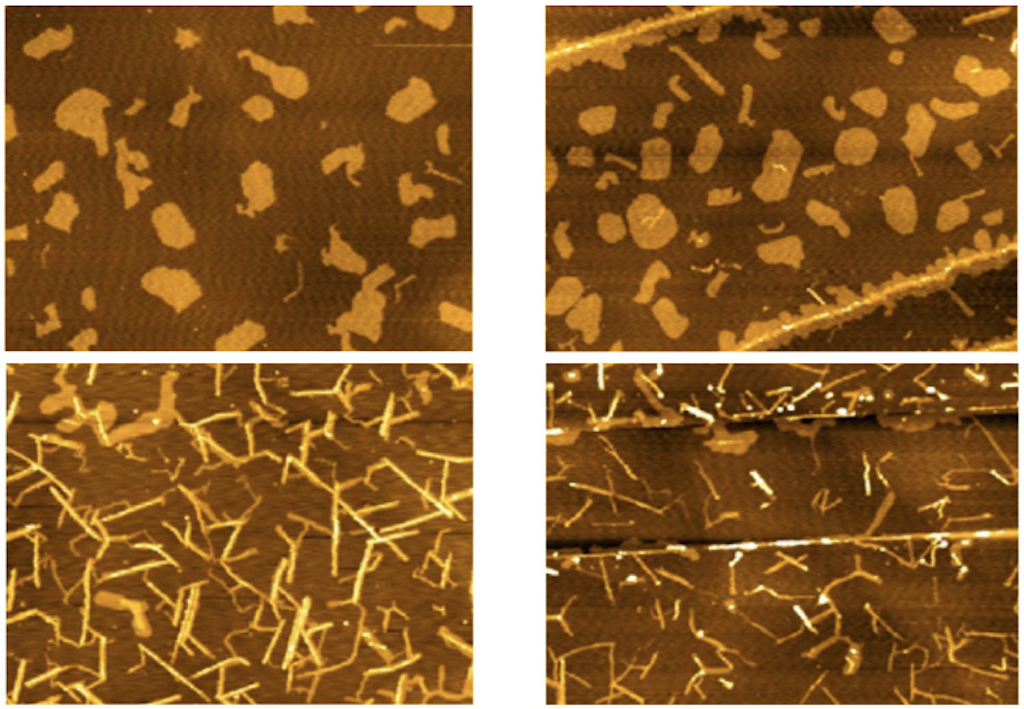
\includegraphics[width=0.6\linewidth]{fabrication.png}
\end{minipage} 
\hspace{-6cm}
\begin{minipage}[c]{0.2\textwidth}
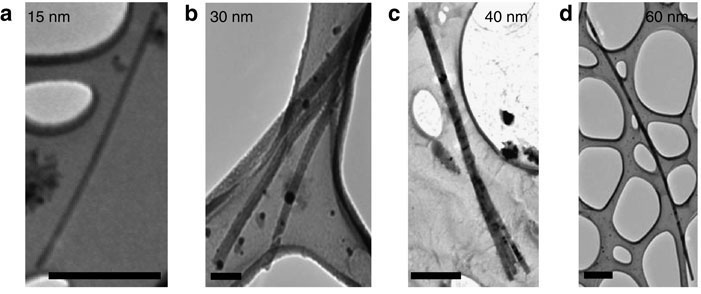
\includegraphics[width=0.9\linewidth]{grapheneNanoribbons.jpg}
\end{minipage}
\caption{\small{Left: Fabrication of TMD nanoribbons. From top to bottom: Atomic Force Microscopy (AFM) images showing nanostructures ranging from 2D nanoislands to nanoribbons (adapted from \cite{chen}). Right: (a) to (d) - Transmission electron microscopy (TEM) images of graphene nanoribbons (GNRs) of widths 15, 30, 40, and 60 $nm$, respectively (adapted from \cite{Mohanty2012} )}. \label{fig:fabrication}}
\end{figure}

A nanoribbon consists of a 2D layer that is much longer on one direction than on the other (Figure \ref{fig:fabrication}), so that edge states become relevant, and can be controlled to yield interesting properties. A high density of low-energy electronic states is localized at the  zigzag edges (Figure \ref{fig:nanoribbons}, left), decaying quickly in the bulk, which suggests the possibility of magnetic ordering. In fact, a mean field solution of the Hubbard model shows that magnetic moments are localized at the edges in graphene \cite{yazyev} (Figure \ref{fig:nanoribbons}, right). QMC has been used to investigate edge-state magnetism beyond mean field in graphene \cite{qmc_results1, qmc_results2, qmc_results3, qmc_results4, qmc_results5}.
However, edge magnetism in TMD nanoribbons remains unexplored \cite{nanoribbon}, and that is one of the goals of this work.
 
\begin{figure}
\begin{minipage}[c]{0.2\textwidth}
\centering
\hspace{-3.5cm}
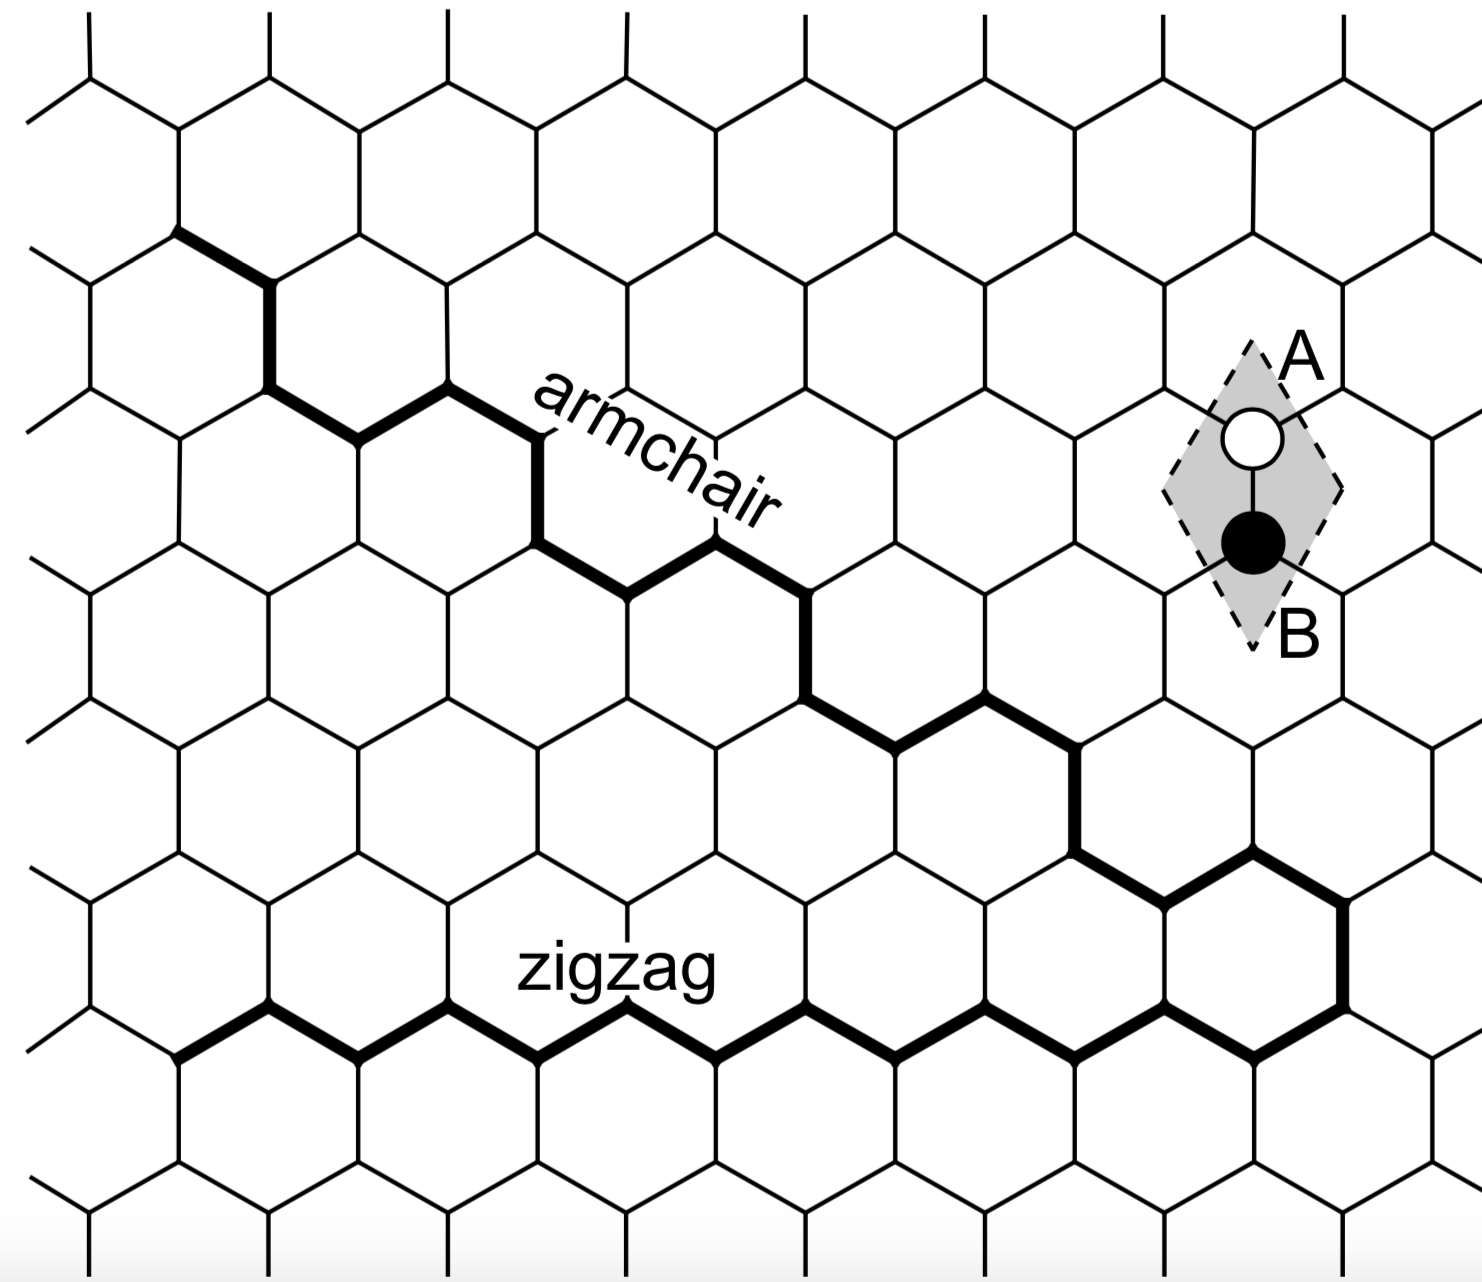
\includegraphics[width=0.65\linewidth]{zigzag}
\end{minipage} \hspace{-2cm}
\begin{minipage}[c]{0.2\textwidth}
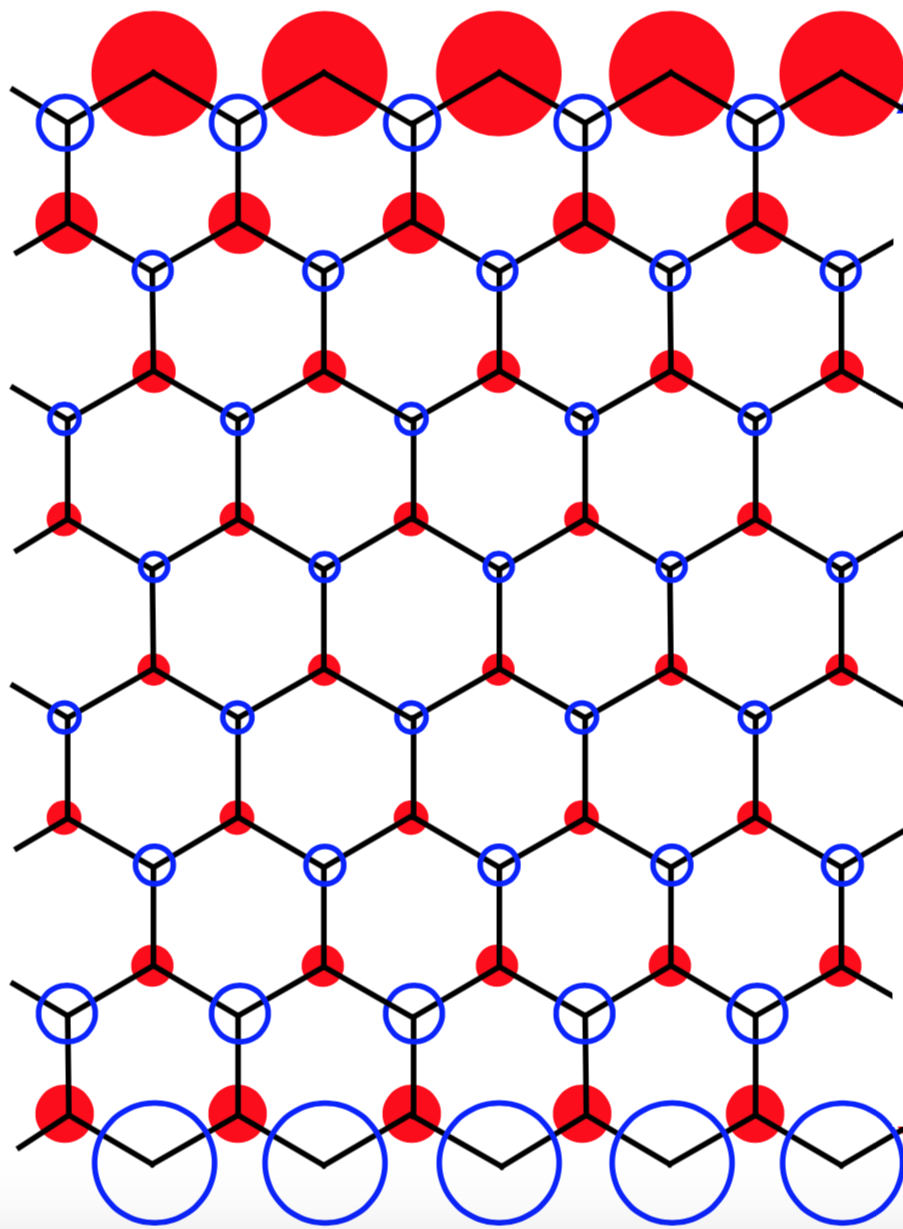
\includegraphics[width=0.45\linewidth]{edge_states}
\end{minipage}
\caption{\small{Left: Two possible terminations of a TMD nanoribbon condensing in a honeycomb lattice. Right: Electronic edge states and the  corresponding local magnetic moments accumulate on the zig zag edges. The area of the circles corresponds to the magnitude of the magnetic moment, while the color red corresponds to a spin up density, and blue to a spin down density \cite{yazyev}.} \label{fig:nanoribbons}}
\end{figure}
\vspace{-1cm}
\section{Method}

Our aim is to apply a QMC code to simulate a 2D TMD nanoribbon. We wish to probe the system for edge-state magnetism, and compare the results with those obtained by a mean field approach, and with those obtained for graphene nanoribbons. To take into account the electron-electron interactions within the nanoribbon, we consider the Hubbard model:
\vspace{-0.3cm}
\begin{equation}\label{eq:hubbard}
\begin{split}
\mathcal{H} &= \underbrace{-t \sum_{\left\langle i, j \right \rangle, \sigma} \bigg( c_{i,\sigma}^\dagger c_{j,\sigma} + c_{j,\sigma}^\dagger c_{i,\sigma} \bigg) -\mu \sum_i \bigg( n_{i,\uparrow} + n_{i,\downarrow} \bigg)}_{\mathcal{H}_0} \\ 
&+\underbrace{U \sum_{i} \bigg( n_{i,\uparrow} - \frac{1}{2} \bigg) \bigg( n_{i,\downarrow} - \frac{1}{2} \bigg)}_{\mathcal{H}_1}
\end{split}
\end{equation}
\vspace{-1cm}

A given physical observable of interest $\mathcal{O}$, such as the spin-spin correlation (that describes the degree of magnetic ordering), or the magnetic susceptibility may be computed formally by
\vspace{-0.5cm}
\begin{equation}\label{eq:observables}
\left\langle \mathcal{O} \right\rangle = \text{Tr} ( \mathcal{O} \mathcal{P} )\, \, , \text{where} \,\, \mathcal{P} \equiv \frac{1}{Z} e^{-\beta \mathcal{H} } , \,\, Z = \text{Tr} ( e^{-\beta \mathcal{H} } ) 
\end{equation}
\vspace{-1cm}

The big idea behind the so called determinantal QMC approach is to map the $d$-dimensional many-body quantum problem onto a $(d+1)$-dimensional classical problem, in terms of which these averages may be evaluated stochastically by a standard Monte Carlo method. We start by rewriting the partition function, invoking an analogy with the computation of the Green's function of a time-evolving quantum system:
\vspace{-0.5cm}
\begin{equation}
Z = \Tr \prod_{l = 1}^L e^{-\Delta \tau \mathcal{H} } =  \Tr \prod_{l = 1}^L e^{-\Delta \tau \mathcal{H}_0}  e^{-\Delta \tau \mathcal{H}_1} + \mathcal{O}(\Delta \tau^2) ,
\end{equation}
where we divided the analogous of an "imaginary time" interval $[0, \beta]$ (in the time-evolving case) into $L$ equal sub-intervals of width $\Delta \tau = \beta / L$. The error arising in the second step is controlled: for small $\Delta \tau$, the truncation is a good approximation, and we are able to factorize the contributions of the quadratic and quartic terms by ignoring the contributions of terms containing their commutators. This is called the Trotter breakup and $\Delta \tau$ is the Trotter error.

The first step is to recast the quartic $U$-term of equation (\ref{eq:hubbard}) in quadratic form. This is convenient because a known theorem for quadratic Hamiltonians of type $\mathcal{H}_l = \sum_{\alpha,\beta} c_{\alpha}^\dagger (H_l)_{\alpha\beta} c_{\beta}$, where $H_l$ is a real matrix, allows us to take the trace in equation (\ref{eq:observables}):
\vspace{-0.3cm}
\begin{equation}
\Tr ( e^{-\mathcal{H}_1} e^{-\mathcal{H}_2} ... e^{-\mathcal{H}_L}) = \det ( I + e^{-H_L} e^{-H_{L-1}} ... e^{-H_1} )
\end{equation}

The advertised quadratic term is obtained by performing a so called discrete Hubbard-Stratonovich (HS) transformation. The price to pay is that the system becomes coupled to a discrete, spatially varying external field, $[h_i]$. Additionally, the HS field can only take on the values $\pm 1$, which effectively makes it a field of Ising spins, and it is defined for each imaginary time slice, so that it actually becomes a matrix $\bm h = [ h_{l, i} ]$. The upshot is that after some algebra, we obtain the distribution function of the $(d+1)$-dimensional (the extra dimension is the "imaginary time") classical system corresponding to our interacting $d$-dimensional quantum system:
\vspace{-0.5cm}
\begin{equation}
P ( \bm h ) \propto \det [ \bm M_{\uparrow} ( \bm h ) ] \det [ \bm M_{\downarrow} ( \bm h )  ] ,
\end{equation}
where $\bm M_{\uparrow}$ corresponds to the spin-up sector, and $\bm M_{\downarrow}$ corresponds to the spin-down sector. Apart from depending on $\bm h$, the $\bm M$-matrices depend on: the parameters of the model $t, U, \mu$, the geometry of the lattice, and the Trotter error $\Delta \tau$. Once we fix those, the $\bm M$-matrices only depend on the HS field, $\bm h$. This makes it possible to sample configurations of the system using, for example the Metropolis-Hastings algorithm: start with a random $\bm h$, and flip "spins", either accepting or rejecting moves in an adequate way so as to ultimately draw random samples from $P (\bm h)$. As we sample configurations of the system, we can compute averages of observables of interest, probing the system for magnetic, charge, or superconducting order. This method is the current state-of-the-art, allowing us to efficiently circumvent a variety of numerical issues: the efficient sampling of HS-field configurations, the stabilization of the simulation at low temperature, and the fermion sign problem. The latter is due to the antisymmetry of the many-fermion wave function, leading to the appearance of negative statistical weights $P ( \bm h) < 0$ that severely hinder the computation of averages of the relevant observables.

%---------------------------------------------------------------------------
% --- Bibliography
%---------------------------------------------------------------------------
\vspace{-1cm}
\bibliographystyle{plain}
\bibliography{sample.bib}
\vspace{-1.5cm}
\section{Acknowledgements}

The work at CFP is suported by the FCT grant UID/FIS/04650/2013.
\vspace{-1cm}
\begin{figure}
\raggedleft

\includegraphics[scale=0.7]{fct.png}
\end{figure}

\end{multicols}

% Make a footer line/box:
\makefooter



\end{document}





